% Created 2024-03-30 Sat 14:54
% Intended LaTeX compiler: pdflatex
\documentclass[11pt]{article}
\usepackage[utf8]{inputenc}
\usepackage[T1]{fontenc}
\usepackage{graphicx}
\usepackage{longtable}
\usepackage{wrapfig}
\usepackage{rotating}
\usepackage[normalem]{ulem}
\usepackage{amsmath}
\usepackage{amssymb}
\usepackage{capt-of}
\usepackage{hyperref}
\author{W}
\date{\today}
\title{ISYE 7406: Data Mining and Statistical Learning}
\hypersetup{
 pdfauthor={W},
 pdftitle={ISYE 7406: Data Mining and Statistical Learning},
 pdfkeywords={},
 pdfsubject={},
 pdfcreator={Emacs 28.1 (Org mode 9.5.2)},
 pdflang={English}}
\begin{document}

\maketitle
\tableofcontents

\section{Bootstrapping algorithm}
\label{sec:org8d67579}
9.1.3
\subsection{Motivating example}
\label{sec:org8240330}
\begin{itemize}
\item Data: \(z = (z_1, ..., z_n)\) where \(z_i = (Y_i, x_{i1}, ..., x_{ip}), i=1,...,n\)
\item Parameter estimation: we derived real-valued summary statistics
\(S(z) = S(z_1, ..., z_n)\) which is en estimator of population parameter \(\theta\) (e.g. mean, median, correlation coefficient, regression coefficient, etc.)
\item Objective: derive a \textbf{\textbf{robust}} estimator of the confidence interval of \(\theta\) or the standard error of \(S(z)\)
\item Challenges: we don't know the distribution of data, and are unable to obtain additional training datasets
\end{itemize}
\subsection{Idea in Bootstrapping algorithm}
\label{sec:org4df9d32}
\begin{itemize}
\item Intuitive idea:
\begin{itemize}
\item Estimate the standard error of \(S(z) = S(z_1, ..., z_n)\) based on the sample standard deviation if we have many values of \(S(z)\) or many independent copies of training data
\item from the original training dataset (\(z= z_1, z_2, ..., z_n\)) to generate many copies of "new" training dataset. This allows us to compute many values of \(S(z)\)
\end{itemize}
\end{itemize}
\subsection{Resample with replacement}
\label{sec:orgc71a823}
\begin{center}
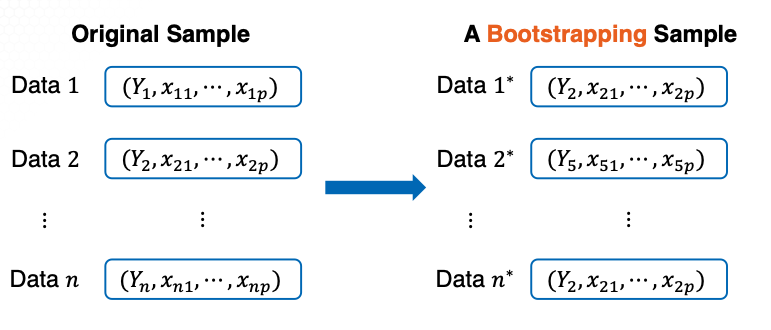
\includegraphics[width=.9\linewidth]{./img/bootstrap-resample.png}
\end{center}
\begin{itemize}
\item High level:
\begin{itemize}
\item Input Data: \(z = (z_1, ..., z_n)\) where \(z_i = (Y_i, x_{i1}, ..., x_{ip}), i=1,...,n\) and estimator of \(S(z)\) for \(\theta\)
\item For \(b=1,...,B\)
\begin{itemize}
\item \textbf{\textbf{Sample with replacement}} to get bootstrap sample \(z^{*b} = (z_1^{*b}, ..., z_n^{*b})\)
\item Compute the value \(S(z^{*b}) = S(z_1^{*b}, ..., z_n^{*b})\) for this bootstrap sample
\end{itemize}
\item Once the \(B\) values of \(S(z^{*b})\) have been computed,
\begin{itemize}
\item The quantiles of \(S(z^{*b})\)'s provide an empirical distribution of \(S(z)\)
\item They can be used to provide confidence intervals of \(\theta\)
\end{itemize}
\end{itemize}
\end{itemize}
\end{document}
